% Asset ID: AS1TrigonometricRatiosTIKZ-001
% Source: P1-Chp9 p.4
% Related section: Prerequisite Recap
% Purpose: Right triangle side labels
\documentclass[tikz,border=8pt]{standalone}
\usepackage{amsmath}
\usetikzlibrary{angles,quotes,calc,arrows.meta}
\begin{document}
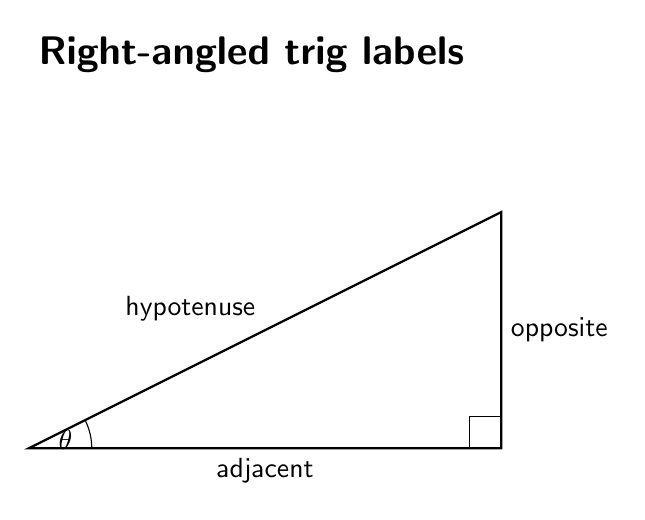
\begin{tikzpicture}[scale=1.0, every node/.style={font=\sffamily}]
\node[font=\sffamily\bfseries\Large, anchor=west] at (0,5) {Right-angled trig labels};
\coordinate (A) at (0,0);\coordinate (B) at (6,0);\coordinate (C) at (6,3);\draw[thick] (A)--(B)--(C)--cycle;\draw (B)--++(-.4,0)--++(0,.4)--++(.4,0);\pic[draw,"$\theta$",angle radius=.8cm] {angle=B--A--C};\node[below] at ($(A)!0.5!(B)$) {adjacent};\node[right] at ($(B)!0.5!(C)$) {opposite};\node[above left] at ($(A)!0.5!(C)$) {hypotenuse};
\end{tikzpicture}
\end{document}
